\renewcommand{\captiontitle}{\UNet{} module}
\begin{figure}
\centering
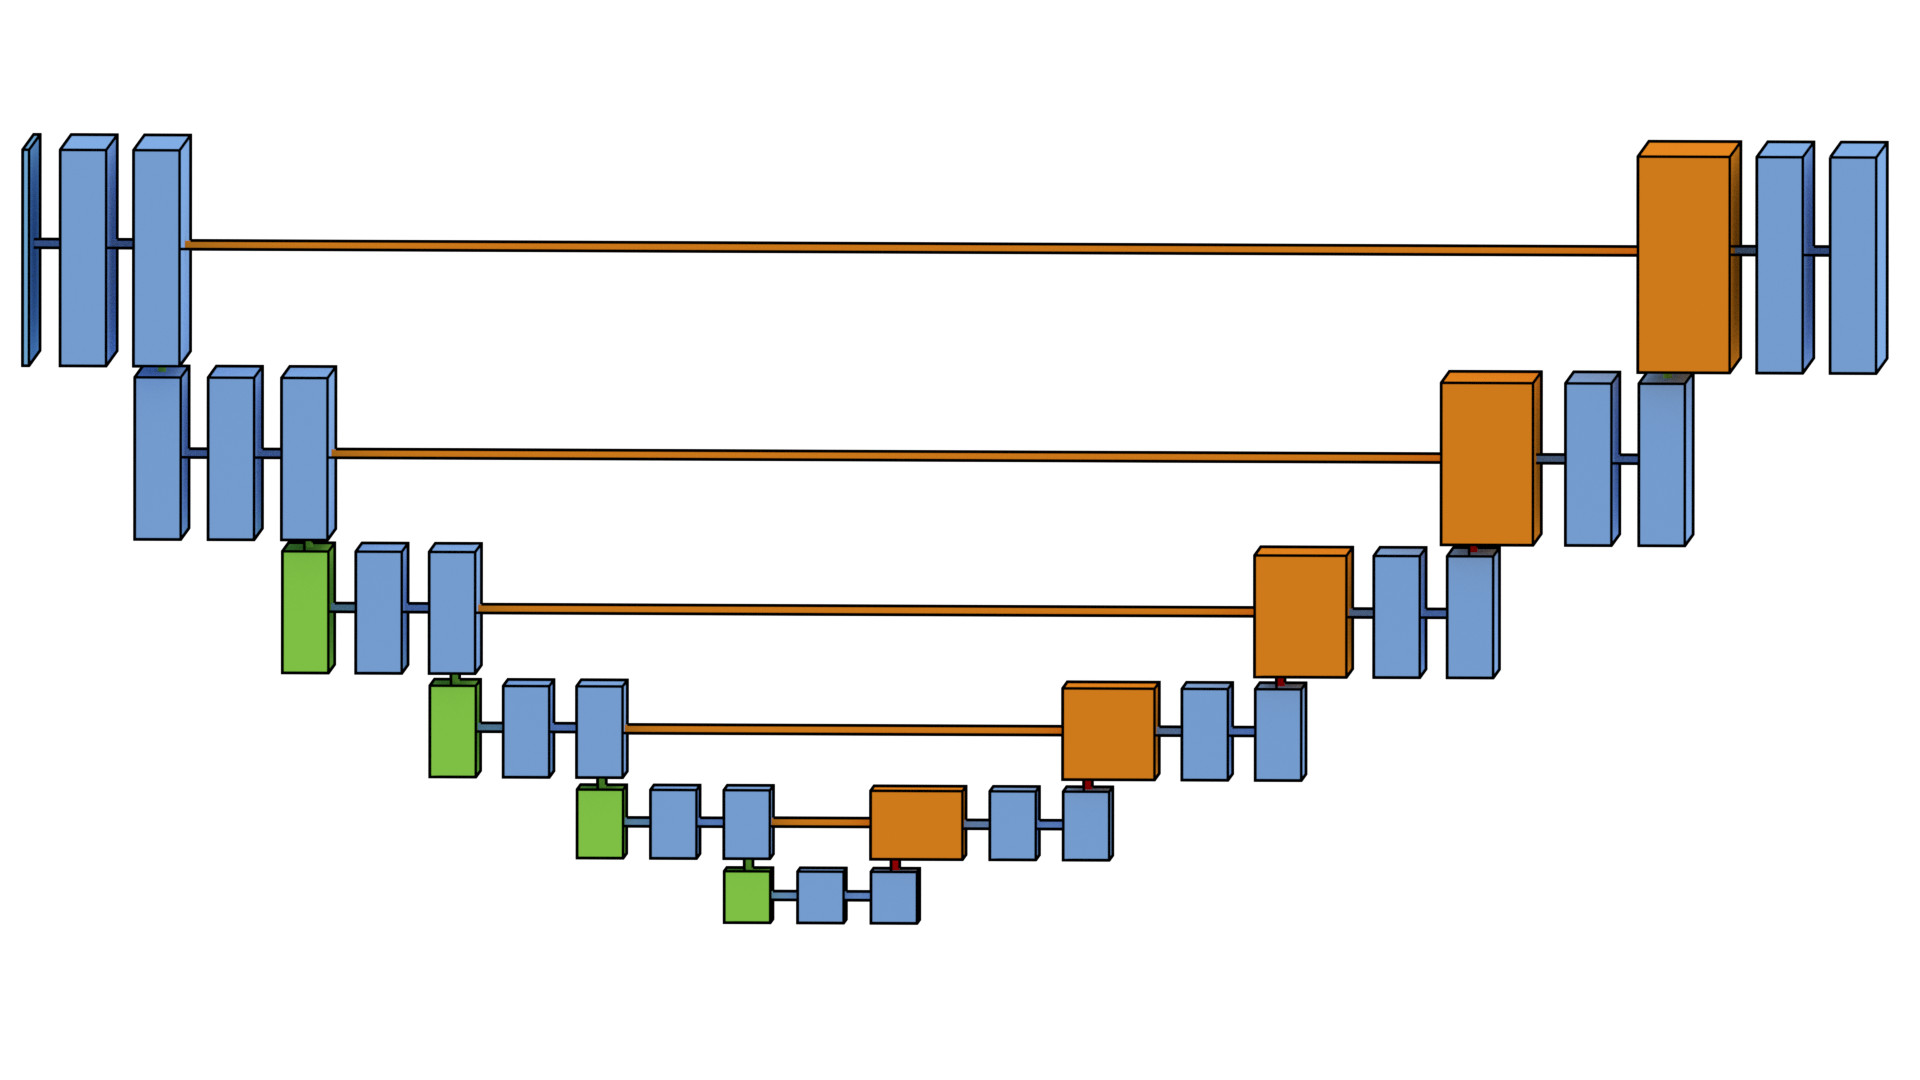
\includegraphics[clip, trim=0 0 0 0,width=0.5\textwidth]{./data/unet-module.png}
\caption[\captiontitle]{\captiontitle{}.  The input image is of size $\N \times \N \times N$, where $N$ is the number of channels ($1$ for all networks).  
\hl{Blue, green, and orange boxes correspond to multichannel feature maps.  Green indicates a downsampled feature map.  Orange indicates the result of a copy, concatenated with an upsampled feature map}.}
\label{fig:unet-module}
\end{figure}

